\documentclass[11pt]{article}
\usepackage[T1]{fontenc}
\usepackage[utf8]{inputenc}
\usepackage[margin=1in]{geometry}
\usepackage{booktabs,amsmath,amssymb,microtype}
\usepackage{hyperref,graphicx,placeins}
\hypersetup{hidelinks,pdftitle={Reasoning-Trace Distillation under Output Limits: A Qwen3-1.7B Case Study},pdfauthor={Maximilian Ruess}}
\title{Reasoning-Trace Distillation under Output Limits:\\A Qwen3-1.7B Case Study}
\author{Maximilian Ruess}
\date{October 20, 2026}
\begin{document}
\maketitle
\begin{abstract}
An accuracy gain under a short output limit can depend on whether a model reaches its final answer. We study this issue in reasoning-trace distillation into the already post-trained Qwen3-1.7B. An initial experiment fine-tunes three seeds per arm on 500 matched questions with teacher traces or final answers alone. After its 256-question greedy GSM8K evaluation, a separately frozen follow-up evaluates the unchanged student and three trace checkpoints on 128 shared questions at 2K, 4K and 8K with recommended thinking-mode sampling. At 2K, trace checkpoints averaged 80.21\% numerical accuracy versus 67.97\% unchanged. At the follow-up's primary 8K limit, the corresponding accuracies were 86.20\% and 87.50\% (difference -1.30 percentage points; 95\% conditional paired item interval -5.73 to +2.86). The one-box secondary rule reverses the 8K point estimate, but its interval also includes zero. The unchanged student's sampled no-thinking policy reached 78.91\% at 2K with 237 mean tokens, versus 994 for trace checkpoints. Native no-thinking did not reproduce the original answer-only SFT collapse.
 These results describe completion, response length and final-answer accuracy in one student; they do not establish a general improvement in reasoning ability.
\end{abstract}

\section{Introduction}
Reasoning-trace distillation trains a student on a teacher's worked solutions, with the aim of transferring problem-solving behavior~\cite{stepwise,r1}. For a student that already supports explicit thinking, additional supervision can change how long it generates, whether it completes a response and what answer it produces. Accuracy measured at one output limit combines these effects. A trained model that finishes more often can outperform an unchanged checkpoint under that limit without demonstrating an advantage when more output is allowed.

We examine this distinction in \texttt{Qwen/Qwen3-1.7B}, an already post-trained model with native thinking and no-thinking modes~\cite{qwen}. Both supervised fine-tuning (SFT) arms see the same 500 OpenR1 questions and final answers; one also receives the teacher's explicit thinking. Questions, training seeds and optimizer updates are matched. The answer-only recipe performs poorly, so we retain that result and separately evaluate the existing trace checkpoints against the unchanged student and its native no-thinking mode.

The trace checkpoints had higher numerical accuracy at 2K (80.21\% versus 67.97\%) and generated shorter responses. At 8K, where almost all responses terminated at an end-of-sequence (EOS) token, their mean was 86.20\% versus 87.50\% unchanged. The conditional item interval includes zero under both retained scoring rules. Native no-thinking inference also avoided the severe failure seen after answer-only SFT. Together, these results show how output allowances, final-answer formatting and an existing inference mode change the interpretation of a small trace-distillation experiment.


The original greedy study and the sampled follow-up have distinct primary comparisons. The follow-up was designed after inspecting the original findings and uses previously evaluated questions. Its purpose is to test how the interpretation changes under larger output allowances and native inference controls. The contribution is an empirical case study of an existing distillation recipe, rather than a new training or length-control algorithm.

\section{Related work}
\paragraph{Learning from teacher reasoning.}
Hsieh et al. use teacher rationales as an additional target in a multitask framework~\cite{stepwise}. DeepSeek-R1 reports reasoning distillation into smaller models~\cite{r1}, while s1 combines trace SFT with a test-time intervention that extends or terminates thinking~\cite{simple}. Our student already has a trained thinking mode, so the experiment measures additional adaptation of that checkpoint. Li et al. find that students with at most three billion parameters do not consistently benefit from longer or stronger-teacher reasoning and propose mixing supervision of different complexity~\cite{small}. We use one fixed teacher-trace selection; we do not compare short and long teacher traces.

\paragraph{Reasoning length and inference policy.}
Chen et al. study overthinking and use self-training to shorten reasoning while preserving accuracy~\cite{overthinking}. Aggarwal and Welleck introduce Length Controlled Policy Optimization (LCPO), which trains L1 to satisfy a requested length constraint while optimizing accuracy~\cite{l1}. These methods explicitly target the allocation of reasoning length. Our trace SFT has no length-control objective or inference-time budget forcing: generation stops at an end token or a fixed ceiling. We examine completion and final-answer accuracy under those ceilings, including the student's existing no-thinking policy.

\section{Experimental design}
\label{sec:distillation}
\subsection{Matched training questions and supervision}
\paragraph{Student and matched supervision.}
The student is a pinned revision of the post-trained \texttt{Qwen/Qwen3-1.7B} checkpoint. Both arms use the same 500 questions and existing DeepSeek-R1 teacher generations from OpenR1-Math-220k~\cite{data}. Eligible generations have a positive dataset correctness-verification flag, a complete thinking block, a final boxed value and a complete serialized target within 16,128 tokens. This reserves instruction space under the 16,384-token training ceiling. Exact and near-duplicate overlap candidates against GSM8K and MATH-500 test questions are removed before selection~\cite{gsm,math}. Verification labels come from the dataset; they were not independently reviewed by humans.

The answer-only arm receives the final boxed value. The trace arm receives the teacher's \texttt{<think>} block, unchanged apart from outer whitespace, followed by the identical box. Post-thinking prose is removed from both arms, and final fields are normalized to the same box. Both arms receive the same question and final-answer instruction. The selected answers include numeric and symbolic values; their composition and exact prompt are given in Appendix~\ref{app:details}.

The Qwen3 chat template inserts an empty thinking block before each answer-only assistant target. The prepared completion masks supervise these markers in all 500 answer-only examples. Trace targets instead supervise the teacher's populated thinking block. This template behavior is part of the compared recipe.

\begin{table}[ht]
\centering\small
\begin{tabular}{lrrr}
\toprule
Supervision & Questions & Input tokens/epoch & Supervised tokens/epoch \\
\midrule
Final answer only & 500 & 63,828 & 7,377 \\
Teacher thinking plus final answer & 500 & 2,691,567 & 2,635,116 \\
\bottomrule
\end{tabular}
\caption{Training token exposure per epoch. Complete targets retain their end-of-turn token. Questions and updates are matched across arms; token exposure and compute differ.}
\label{tab:distill-exposure}
\end{table}

\paragraph{Training.}
Each arm uses seeds 42, 43 and 44, two epochs and 64 optimizer updates, with the same seeded question minibatches. Training uses rank-64 rsLoRA and completion-only loss. Questions and updates are matched, while token exposure and compute differ substantially (Table~\ref{tab:distill-exposure}). Other hyperparameters are listed in Appendix~\ref{app:details}.

\subsection{Original greedy evaluation}
The unchanged student and all six trained checkpoints receive the same 256 frozen GSM8K test questions~\cite{gsm}, with thinking enabled, greedy decoding and a 2,048-token output limit (2K). Selection excludes earlier development and checkpoint-ablation questions. Before generation, 64 of these questions are selected for a 4,096-token check (4K) on all seven checkpoints. The original primary comparison is mean trace-minus-answer-only numerical accuracy at 2K. Comparisons with the unchanged student and the 4K check are secondary or descriptive. The protocol and numerical rule were fixed before these generations.

\subsection{Sampled inference follow-up}
After reviewing the original results, a separate protocol froze 128 of its 256 questions. The unchanged student and three existing trace checkpoints each receive one sampled generation per question at 2K, 4K and 8,192 tokens (8K). Qwen's model card advises against greedy thinking-mode decoding; the follow-up uses its recommended temperature 0.6, top-p 0.95, top-k 20 and disabled min-p~\cite{qwen}. The decoding seed is fixed. A common generated-token memory ceiling gives batches of 32, 16 and 8 across the three limits. Batch membership determines random-number seeds, so the runs are separately sampled trajectories rather than prefixes of one shared rollout.

Two unchanged-student no-thinking controls use the same 128 questions at 2K. One uses the recommended no-thinking sampling policy, temperature 0.7, top-p 0.8 and top-k 20, with disabled min-p. The other uses greedy decoding to compare with the original answer-only outputs. Both retain the common final-answer instruction. Original greedy records are restricted to these exact questions rather than regenerated.

The follow-up primary comparison, fixed before its generations, is mean trace-minus-unchanged numerical accuracy at 8K. Outcomes at 2K/4K, no-thinking controls, strict scores and completion or length diagnostics are secondary or descriptive. This development-informed follow-up preserves the original primary comparison and runs no new training.

\subsection{Scoring and uncertainty}
The numerical primary rule excludes any balanced thinking blocks and grades the remaining final response. It requires at least one complete numeric box and accepts repeated boxes only when their values are numerically identical. Missing, malformed, conflicting or nonnumeric final boxes and unfinished or malformed thinking fail; integer gold answers compare exactly. The strict secondary rule additionally requires exactly one box. In native no-thinking mode, the chat template supplies an empty closed thinking block in the prompt. End-of-sequence (EOS) termination is recorded separately: a response can close its thinking block and still reach the output limit. Lengths count generated thinking and final-response tokens.

For each comparison, we average the three trained-checkpoint correctness differences within each question, then draw 10,000 paired question-bootstrap resamples with seed 42. Reported 95\% intervals describe item uncertainty conditional on the observed checkpoints and, for the sampled follow-up, the decoding seed. Training-seed difference standard deviations are reported separately. Three checkpoints on 128 shared questions do not constitute 384 independent items. The original protocol uses the same calculation on its 256 questions. Raw outputs retain both scoring rules and were checked for persistence and CPU strict-score reproduction.


\section{Sampled inference results}
\label{sec:followup}
\subsection{Accuracy across output limits}
Trace checkpoints averaged 80.21\% accuracy at 2K, compared with 67.97\% for the unchanged student, a descriptive difference of +12.24 percentage points. The corresponding differences at 4K and 8K were -1.30 and -1.30 points (Table~\ref{tab:followup-accuracy}).
\par\begin{table}[ht]\centering\small\begin{tabular}{llrrr}\toprule
Checkpoint & Training seed & 2K (\%) & 4K (\%) & 8K (\%) \\
\midrule
Unchanged & -- & 67.97 & 85.94 & 87.50 \\
Teacher trace & 42 & 80.47 & 82.81 & 86.72 \\
Teacher trace & 43 & 82.03 & 83.59 & 85.94 \\
Teacher trace & 44 & 78.12 & 87.50 & 85.94 \\
Trace mean & -- & 80.21 & 84.64 & 86.20 \\
Trace mean $-$ unchanged & -- & +12.24 & -1.30 & -1.30 \\
\bottomrule\end{tabular}\caption{Numerical primary accuracy on the same 128 questions at each output limit. The trace mean averages three trained checkpoints; the last row gives percentage-point differences. Thinking-mode sampling uses one fixed decoding seed and effective batches of 32/16/8.}\label{tab:followup-accuracy}\end{table}\par
At the follow-up's primary 8K limit, trace checkpoints averaged 86.20\% versus 87.50\% unchanged. The mean difference was -1.30 percentage points (95\% paired item-bootstrap interval -5.73 to +2.86); the training-seed difference SD was 0.45 points. The interval conditions on the three trained checkpoints and the one decoding seed. The 8K numerical comparison establishes neither an accuracy advantage nor equivalence. Comparisons at 2K/4K are descriptive.
\par\begin{figure}[ht]\centering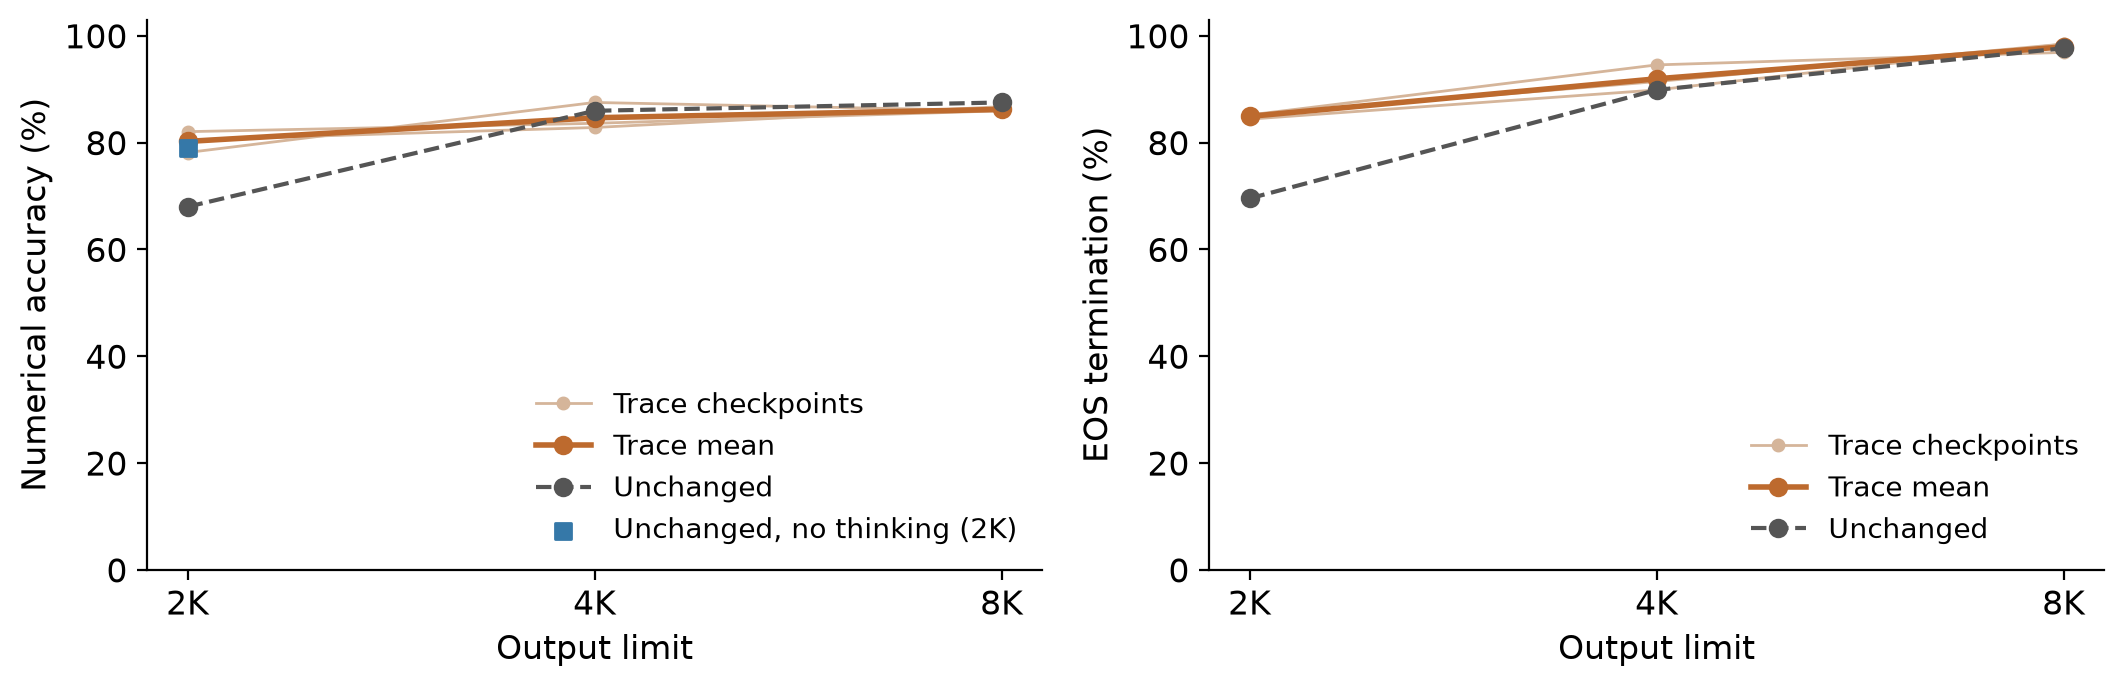
\includegraphics[width=\textwidth]{assets/inference-extension-2026-10-20.png}
\caption{Sampled follow-up on 128 shared questions. Left: numerical accuracy; the blue square is the unchanged student's sampled no-thinking policy, tested only at 2K. Right: fraction terminating at EOS rather than the output limit. Thin orange lines are individual trace checkpoints; thicker lines show their mean. Effective batch size changes with the limit.}\label{fig:followup}\end{figure}\par
\subsection{Sensitivity to final-answer formatting}
Five unchanged-student responses at 8K contain repeated, numerically consistent correct boxes. They pass the numerical primary rule and fail the exactly-one-box secondary rule. The trace scores are unchanged. The strict rule therefore reverses the point estimate to +2.60 points, with a conditional item interval of -2.60 to +8.07 (Table~\ref{tab:format-sensitivity}). Neither rule establishes an 8K advantage. The primary rule was fixed before the follow-up generations and is retained throughout.
\par\begin{table}[ht]\centering\small\begin{tabular}{lrrr}\toprule
8K scoring rule & Unchanged (\%) & Trace mean (\%) & Difference (pp) \\
\midrule
Numerical, primary & 87.50 & 86.20 & -1.30 \\
One box, secondary & 83.59 & 86.20 & +2.60 \\
\bottomrule\end{tabular}\caption{The same 128 questions and raw generations, scored under two prospectively retained rules. The numerical primary accepts repeated identical numeric boxes; the strict secondary requires exactly one box. Differences are trace mean minus unchanged.}\label{tab:format-sensitivity}\end{table}\par
\subsection{Completion and response length}
At 2K, 69.53\% of unchanged-student responses ended at an end-of-sequence (EOS) token, compared with 84.90\% across trace checkpoints. Mean generated lengths were 1451 and 994 tokens, respectively. At 8K, EOS rates were 97.66\% and 97.92\%; trace checkpoints still generated fewer tokens on average (1520 versus 2012; Table~\ref{tab:followup-completion}). These lengths include all generated thinking and final-response tokens, subject to the stated limits.
\par\begin{table}[ht]\centering\small\begin{tabular}{llrrrr}\toprule
Checkpoint & Seed & Correct/128 & EOS (\%) & Unfinished (\%) & Tokens \\
\midrule
Unchanged & -- & 112 & 97.66 & 2.34 & 2012 \\
Teacher trace & 42 & 111 & 98.44 & 1.56 & 1511 \\
Teacher trace & 43 & 110 & 98.44 & 1.56 & 1575 \\
Teacher trace & 44 & 110 & 96.88 & 3.12 & 1473 \\
\bottomrule\end{tabular}\caption{Completion and mean generated tokens at 8K. Unfinished denotes an unclosed thinking block, which is distinct from EOS termination. Missing or invalid final fields remain incorrect.}\label{tab:followup-completion}\end{table}\par
\subsection{Native no-thinking inference and the failed training control}
Disabling the unchanged student's thinking channel yielded 77.34\% accuracy with greedy decoding and 78.91\% with its recommended sampled policy. The original answer-only checkpoints averaged 6.51\% under greedy decoding on these exact 128 questions. Native no-thinking therefore did not reproduce the answer-only SFT collapse (Table~\ref{tab:nothinking}). Both native no-thinking runs terminated at EOS on all 128 questions.
\par\begin{table}[ht]\centering\small\begin{tabular}{llrr}\toprule
Checkpoint or recipe & Decoding & Accuracy (\%) & Mean tokens \\
\midrule
Unchanged, no thinking & greedy & 77.34 & 239 \\
Unchanged, no thinking & sampled & 78.91 & 237 \\
Unchanged, thinking & greedy & 74.22 & 1386 \\
Answer-only SFT, seed 42 & greedy & 5.47 & 12 \\
Answer-only SFT, seed 43 & greedy & 7.03 & 11 \\
Answer-only SFT, seed 44 & greedy & 7.03 & 11 \\
\bottomrule\end{tabular}\caption{All entries use the same 128 questions at 2K. Greedy thinking and answer-only entries are retained original outputs on this subset, not reruns. The no-thinking sampled policy uses temperature 0.7 and top-p 0.8; it must not be treated as decoder-matched to greedy outputs.}\label{tab:nothinking}\end{table}\par
The sampled native policy used 237 mean tokens, compared with 994 for trace checkpoints at 2K, with accuracies of 78.91\% and 80.21\%. This is a descriptive comparison of complete inference recipes: thinking and no-thinking use different sampling parameters. Disabling the explicit thinking channel also permits worked steps in the final response; it does not imply an absence of reasoning.

\FloatBarrier

\section{Original greedy results and completion diagnostic}
\label{sec:original}
\par\begin{table}[ht]\centering\small\begin{tabular}{llrrr}\toprule
Checkpoint & Seed & Correct/256 & Accuracy (\%) & Tokens \\
\midrule
Unchanged & -- & 180 & 70.31 & 1436 \\
Answer only & 42 & 15 & 5.86 & 12 \\
Teacher trace & 42 & 197 & 76.95 & 974 \\
Answer only & 43 & 16 & 6.25 & 12 \\
Teacher trace & 43 & 207 & 80.86 & 956 \\
Answer only & 44 & 17 & 6.64 & 11 \\
Teacher trace & 44 & 196 & 76.56 & 1034 \\
\bottomrule\end{tabular}\caption{Original numerical outcomes on 256 common GSM8K questions with greedy thinking and a 2K limit. All seven checkpoints use the same questions.}\label{tab:original}\end{table}\par
The original primary trace-minus-answer difference was +71.88 percentage points (95\% conditional item interval +67.06 to +76.56; seed-difference SD 2.44 points). Trace SFT averaged 78.12\%, answer-only SFT 6.25\% and the unchanged student 70.31\%. The separate descriptive trace-minus-unchanged difference was +7.81 points (conditional interval +3.39 to +12.50). The unchanged student's strict score was 176/256; strict and numerical scores coincide for the other six checkpoints.

All 768 answer-only outputs contained empty visible thinking blocks. The recipe's large deficit limits interpretation of the primary contrast. An original preselected 64-question greedy check at 4K yielded a trace mean of 83.85\% versus 87.50\% unchanged, a descriptive difference of $-3.65$ points (conditional interval $-8.33$ to $+1.04$). This check uses a different subset and greedy decoding, rather than the follow-up's sampled policy.

\subsection{Post hoc completion diagnostic for the original 2K evaluation}
Among the 101 question--seed pairs where a trace checkpoint was correct and the unchanged student was incorrect, the unchanged response hit the output limit in 99 pairs. These pairs reuse the same 256 questions across training seeds. Conversely, there were 41 unchanged-only correct pairs, of which 29 involved an output-limited trace response. Most trace-only correct pairs thus involve an output-limited unchanged response, while leaving unknown how those responses would have answered with more generation.
\par\begin{table}[ht]\centering\small\begin{tabular}{lrr}\toprule
Original 2K subset & Unchanged & Trace, pooled \\
\midrule
EOS-terminated & 180/184 (97.83\%) & 600/641 (93.60\%) \\
No unfinished thinking & 180/193 (93.26\%) & 600/642 (93.46\%) \\
\bottomrule\end{tabular}\caption{Correct responses divided by each model-dependent subset, with conditional accuracy in parentheses. Trace pooling reuses 256 questions across three checkpoints. Closing a thinking block does not imply EOS termination; these selected subsets do not isolate reasoning ability.}\label{tab:original-completion}\end{table}\par

\FloatBarrier

\section{Discussion}
The trace checkpoints' shorter responses are accompanied by a numerical accuracy advantage at the 2K limit, where the unchanged student often fails to terminate. At 4K and 8K its numerical point estimate is higher. This pattern, together with the original-output diagnostic, supports completion behavior as an important part of the short-limit result. It does not identify how a truncated response would have answered if continued.

Long supervision also coexists with shorter student outputs. The serialized trace-arm targets average 5270 supervised tokens per example; at 8K the students generate 1520 tokens on average, versus 2012 unchanged. The training and test tasks differ, and teacher length was not varied. These observations do not establish that the student learned to compress the teacher's reasoning.

The no-thinking controls change the interpretation of the failed answer-only arm. Switching off the native thinking channel is insufficient to reproduce its collapse. They also provide a practical baseline for short-output use: the sampled native policy's observed accuracy is close to the 2K trace mean and its responses are much shorter. The policy comparison remains descriptive; token counts alone do not measure latency or proportional GPU-cost savings.


\section{Limitations}
\paragraph{Sample and generalization.}
The study covers one student, one 500-question training sample and GSM8K. No second benchmark, model-size comparison or teacher-length ablation was run. GSM8K had already been used in this repository, and the follow-up reuses questions from the original evaluation. Training-data overlap screening and the exclusion of recent development questions do not establish a hidden or uncontaminated test. The 128-question follow-up and three trained seeds leave substantial uncertainty: the numerical primary interval at 8K permits effects from a 5.73-point loss to a 2.86-point gain.

\paragraph{Training control.}
The trace arm receives far more supervised tokens and compute despite matched questions and updates. The answer-only results concern one template, learning rate and update schedule. Native no-thinking shows that disabling the explicit thinking channel alone does not reproduce its failure, but it cannot identify the roles of output-style learning, knowledge forgetting or other training effects. No alternative answer-only template or hyperparameter sweep was evaluated.

\paragraph{Inference and measurement.}
The original greedy policy conflicts with Qwen's thinking-mode guidance; the follow-up uses its recommended sampling parameters. Even the 8K ceiling remains below the model card's recommended 32,768-token allowance~\cite{qwen}. One decoding seed does not estimate variability across sampled generations. Batch size and random-number streams also change across output limits, preventing an isolated causal estimate of the ceiling's effect. Bootstrap intervals condition on the observed checkpoints and decoding seed. Conditional completion rates select different questions for each model, and final-answer scoring does not measure the correctness or faithfulness of the intermediate reasoning.

\section{Conclusion}
In this Qwen3-1.7B case study, trace SFT produced shorter observed GSM8K responses and higher numerical accuracy at the 2K limit. The 8K numerical comparison establishes neither an accuracy advantage nor equivalence. The strict one-box secondary rule changes the 8K point estimate's sign without establishing an advantage. Native no-thinking inference did not reproduce the answer-only SFT collapse. Evaluating trace distillation in this setting therefore requires output-budget comparisons, explicit scoring rules and native inference controls alongside the trained checkpoints.


\paragraph{Artifacts.}
The repository retains the questions, protocols, code and model identities, raw generations and both scoring endpoints. Saved generations passed persistence checks and strict scores reproduce on CPU. Trained weights remain on the persistent experiment volume and have not been publicly released. Historical recipe rankings and checkpoint-repair records are documented separately from the experiments reported here.

\begin{thebibliography}{12}
\raggedright\small
\bibitem{qwen} Qwen Team. Qwen3 Technical Report. \emph{arXiv:2505.09388}, 2025. Model and inference guidance: \url{https://huggingface.co/Qwen/Qwen3-1.7B}.
\bibitem{stepwise} Cheng-Yu Hsieh et al. Distilling Step-by-Step! Outperforming Larger Language Models with Less Training Data and Smaller Model Sizes. \emph{Findings of ACL}, 2023, pp. 8003--8017. \url{https://aclanthology.org/2023.findings-acl.507/}.
\bibitem{r1} DeepSeek-AI. DeepSeek-R1: Incentivizing Reasoning Capability in LLMs via Reinforcement Learning. \emph{arXiv:2501.12948}, 2025.
\bibitem{small} Yuetai Li et al. Small Models Struggle to Learn from Strong Reasoners. \emph{arXiv:2502.12143}, 2025. \url{https://arxiv.org/abs/2502.12143}.
\bibitem{overthinking} Xingyu Chen et al. Do NOT Think That Much for 2+3=? On the Overthinking of o1-Like LLMs. \emph{arXiv:2412.21187}, 2024. \url{https://arxiv.org/abs/2412.21187}.
\bibitem{l1} Pranjal Aggarwal and Sean Welleck. L1: Controlling How Long A Reasoning Model Thinks With Reinforcement Learning. \emph{COLM}, 2025. \url{https://arxiv.org/abs/2503.04697}.
\bibitem{simple} Niklas Muennighoff et al. s1: Simple test-time scaling. \emph{arXiv:2501.19393}, 2025. \url{https://arxiv.org/abs/2501.19393}.
\bibitem{data} OpenR1-Math-220k. \url{https://huggingface.co/datasets/open-r1/OpenR1-Math-220k}.
\bibitem{gsm} Cobbe et al. Training Verifiers to Solve Math Word Problems. \emph{arXiv:2110.14168}, 2021.
\bibitem{math} MATH-500. \url{https://huggingface.co/datasets/HuggingFaceH4/MATH-500}.
\bibitem{trl} Hugging Face. TRL v0.28.0. \url{https://github.com/huggingface/trl/tree/v0.28.0}.
\end{thebibliography}
\clearpage
\appendix
\section{Training and evaluation details}
\label{app:details}
The student revision is \texttt{70d244cc86ccca08cf5af4e1e306ecf908b1ad5e}. Training seeds are 42/43/44; question-selection seeds are 20261020 for the original 256, 20261021 for its 64-question check, and 20261022 for the follow-up 128. The follow-up's decoding seed is 20261023. The original study generated 2,240 responses; the inference-only follow-up generated 1,792. Original scores remain unchanged.

The selected teacher answers comprise 313 numeric and 187 symbolic or other values. Fifty original teacher final fields contained multiple boxes; both training arms use the same normalized final box. The original GSM8K selection excludes 32 earlier development questions and 256 checkpoint-ablation questions. The original greedy evaluations use batches of 32 at 2K and 16 at 4K.

Training uses four questions per microbatch and up to four accumulation microbatches per optimizer update. Packing is disabled; padding-free FlashAttention resets positions at example boundaries. Both arms use BF16 weights, rank-64 rsLoRA with alpha 64 and dropout 0.05, a learning rate of $2\times10^{-4}$, a linear schedule with 10\% proportional warmup, and eight-bit paged AdamW. Loss is restricted to completion tokens, including the end-of-turn token. The runtime uses TRL 0.28.0~\cite{trl}. Per trained model, two epochs consume 127,656 input and 14,754 supervised tokens in the answer arm, versus 5,383,134 input and 5,270,232 supervised tokens in the trace arm. Complete effective weights are exported after the final update.

Scoring-policy identifiers are \texttt{completed-consistent-numeric-boxes-v1} for numerical results and \texttt{boxed-final-v1} for strict results. The sampled follow-up seeds every canonical batch under \texttt{canonical-batch-v3}. Full execution and checkpoint identities are retained with the raw outputs.

GSM8K evaluation appends the same instruction to every question: ``After your reasoning, put only your final numerical value, with no units or explanation inside exactly one \texttt{\textbackslash boxed\{...\}}.'' Training uses the corresponding instruction requesting a mathematical expression. No-thinking mode is selected through the native chat-template switch; the final-answer instruction is unchanged. The pinned OpenR1 and GSM8K dataset revisions are \texttt{e4e141ec9dea9f8326f4d347be56105859b2bd68} and \texttt{740312add88f781978c0658806c59bc2815b9866}, respectively.

\section{Student-run compute}
The inference follow-up used 6.14 aggregate L40S GPU-call hours across parallel evaluations. Elapsed time priced at the configured GPU, CPU and memory rates gives an estimated \$13.34; including extra startup and incidental allowances gives \$15.47. The original training-and-evaluation study's corresponding resource-time estimate was \$7.01. These estimates exclude upstream generation of the public teacher data and are not reconciled provider invoices. Rates were checked against \url{https://modal.com/pricing} on October 20, 2026.

\end{document}
